%
%  untitled
%
%  Created by Davis Shepherd on 2012-05-22.
%  Copyright (c) 2012 University of Washington. All rights reserved.
%
\documentclass[twocolumn]{article}

% Use utf-8 encoding for foreign characters
\usepackage[utf8]{inputenc}

% Setup for fullpage use
\usepackage{fullpage}

\usepackage{hyperref}

% Uncomment some of the following if you use the features
%
% Running Headers and footers
%\usepackage{fancyhdr}

% Multipart figures
%\usepackage{subfigure}
\usepackage{caption}
\usepackage{subcaption}

% More symbols
%\usepackage{amsmath}
%\usepackage{amssymb}
%\usepackage{latexsym}

% For setting space size
\usepackage{setspace}

% Surround parts of graphics with box
\usepackage{boxedminipage}

% Package for including code in the document
\usepackage{listings}

% If you want to generate a toc for each chapter (use with book)
\usepackage{minitoc}

% This is now the recommended way for checking for PDFLaTeX:
\usepackage{ifpdf}

%\newif\ifpdf
%\ifx\pdfoutput\undefined
%\pdffalse % we are not running PDFLaTeX
%\else
%\pdfoutput=1 % we are running PDFLaTeX
%\pdftrue
%\fi

% For the appendix, inserting the R files verbatim
\usepackage{verbatim}

\ifpdf
\usepackage[pdftex]{graphicx}
\else
\usepackage{graphicx}
\fi
\title{PCA}
\author{ Davis Shepherd \and Jason Uanon \and Yukio Maeda}

\date{\today}

\setstretch{1.5}

\begin{document}

\ifpdf
\DeclareGraphicsExtensions{.pdf, .jpg, .tif}
\else
\DeclareGraphicsExtensions{.eps, .jpg}
\fi

\maketitle


\begin{abstract}
    This paper aims to explore the utility of using Principal Component Analysis (PCA) in conjunction with a naive bayesian learner.  We look at both computation time and accuracy as a way to measure the performance of such a procedure.
\end{abstract}

\section{Introduction} % (fold)
\label{sec:introduction}
Our STAT 391 Project primarily focuses on the statistical analysis of using off-line pattern classification methods to simplify and interpret any given written number sample. Specifically, the project focuses on the implementation and analysis of using one particular method, merging the concepts of Principal Components Analysis (PCA) and Maximum Likelihood Estimation (MLE) within the context of symbol classification to uniquely identify number samples. Additionally, our project tries to determine the relative success of the given method by comparing the resulting numbers (determined by the final calculated likelihoods) with the expected number as well as comparing the likelihood ratio data with that obtained using other handwriting classifiers. 

The idea of character recognition or handwriting recognition as a topic is mainly due to its increased importance within the digital world. Today, many computerized systems depend on character recognition for basic operation including computer tablet software, postal letter software, and bank check processing equipment. While they do correctly recognize symbols most of the time, it still succumbs to failure, diminishing the usefulness of these systems over a long time period. Findings of better classifiers may lead to the method's implementation and a reduction of bad symbol identifications. In addition, the idea of character recognition was motivated by its application within the field of artificial intelligence. In this case, better implementation of algorithms and distinguishing of alphanumeric features could allow for more adaptable models of automated devices, suited to identify and recognize any alphanumeric character.

Handwriting recognition, or the ability to analyze and correctly identify a particular language representation from handwritten graphical marks, has been the topic of much research within the past thirty years due to its complexity and increasing algorithmic development. In contrast to the success of recognizing symbols by human eye, computer recognition software/hardware has had mixed degrees of success mainly because of the variability of each person's symbol-writing characteristics (e.g. size, position, appearance). As a result of the inconsistency of one classifier, researchers have devised numerous algorithms and methods to classify symbols, with most of them comparing current information with that extracted from pre-captured data to make a logical decision. Examples of this other than the highlighted PCA-analysis include the nearest-neighbor algorithm and greedy-point match algorithm. Also, scientists have recently used real-time factors to better determine subtle characteristics of symbols (e.g. pen velocity, stop patterns), improving the overall process by allowing segmentation of visual elements with gathered temporal information. 
% section introduction (end)
\section{Methods} % (fold)
\label{sec:methods}

\subsection{PCA} % (fold)
\label{subsec:pca}
Before we begin to talk about principal component analysis (PCA), we review some basic terminology and results from statistics and linear algebra.\\
The \textbf{expected value} of a discrete data set $X$ (also called the mean) is defined as
\begin{center}
$\displaystyle E[X] = \mu =  \sum_{i=1}^{n}x_ip(x_i)$
\end{center}
For the purposes of this data analysis, we will assume that each data point is equally likely. We'll call the expected value 
$\overline{X}$ and write
\begin{center}
$\displaystyle \overline{X} = \frac{\sum_{i=1}^{n}X_i}{n}$
\end{center}
The \textbf{variance} of a data set $X$ is defined as
\begin{center}
$\displaystyle Var(X) = \sigma^2 = E\left[\left(X-\mu\right)^2\right]$
\end{center} 
and using our above definition for the expected value, we have
\begin{center}
$\displaystyle \sigma^2 = 
\frac{\sum_{i=1}^{n}(X_i - \overline{X})^2}{n-1}$
\end{center}
note that the numerator is $n-1$ instead of $n$ for this formula; this is called the \textbf{sample variance} and is used as an unbiased estimator of the true variance of the data.

With this in mind, let $X$ and $Y$ be two identically distributed sets of data. We define the \textbf{covariance} of $X$ and $Y$ as
\begin{center}
$Cov(X, Y) = 
\frac{\sum_{i=1}^{n}(X_i-\overline{X})(Y_i-\overline{Y})}{n-1}$
\end{center}
Now, suppose we have $n$ identically distributed random variables $X_1, \ldots, X_n$. We define the \textbf{covariance matrix} $\Sigma$ as $\Sigma_{i, j} = Cov(X_i, X_j)$. Note that this matrix is symmetric, which means that it will always have real-valued eigenvalues. These eigenvectors correspond to how the data are related. Essentially, we convert a set of data into a set of orthogonal vectors (the principal compoenents), which means that they are uncorrelated with each other. By ordering the eigenvectors by eigenvalue from highest to lowest, we obtain the components in order of significance. This can be used to reduce the dimensionality of a data set by only selecting a certain amount of the highest-valued components. For example, if we start out with 100 eigenvectors/eigenvalues and we choose only the first 10, then the final data set will only have 10 dimensions.

Each principal component is formed by taking the values of the elements of the eigenvalues as the weights of the linear combination. That is, if each eigenvector has the form
$${\bf e}_{i} = \left(\begin{array}{c} e_{1i} \\ e_{2i} \\ \vdots \\ e_{ni} \end{array}\right)$$
The principal components are formed by:
$$Y_1 = {\bf e}_{11}X_1 + {\bf e}_{21}X_2 + \ldots + {\bf e}_{n1}X_n$$
$$Y_2 = {\bf e}_{12}X_1 + {\bf e}_{22}X_2 + \ldots + {\bf e}_{n2}X_n$$
$$\vdots$$
$$Y_n = {\bf e}_{1n}X_1 + {\bf e}_{2n}X_2 + \ldots + {\bf e}_{nn}X_n$$

PCA, then, can be summarized by following these steps:
\begin{itemize}
    \item Obtain training data and subtract the mean
    \item Calculate the covariance matrix
    \item Calculate its eigenvectors and eigenvalues
    \item Choose components and form a feature vector
    \item Derive a new data set
\end{itemize}
For the last bullet point, the new data set can be created by taking the transpose of the feature ector and multiply it on the left of the original data set:
$$FinalData = RowFeatureVector \times RowDataAdjust$$
where $RowFeatureVector$ is the matrix with the eigenvectors in the columns transposed (so tha the eigenvectors are rows, with the most significant on top) and $RowDataAdjust$ is the mean-adjusted data transposed (so the data are in the columns). 

With this procedure, new data sets are able to be determined with any similarly given data. This reduced feature set is used because otherwise every individual pixel of an image would be considered a separate feature; even for small images, this result in a large number of features that would make computations more difficult. Additionally, performing PCA tells us what the most significant components are. By converting these components into images, this can give us more insight into the structure and correlations of each number.

For our purposes, we will simply be using the built-in \emph{prcomp} method in R to perform PCA. Doing ths minimizes the time spent on technical details and allows us to focus more on the classifying itself. Moreover, it also minimizes the risk of having errors in our own code. This background knowledge about what is going on is essential in order to gain insight into what these principal components mean and how to utilize them.

\subsection{Classification} % (fold)
\label{subsec:classification}
In addition to using PCA, we will also be using a classification scheme to assist in interpreting the various hand-writting image data. Commonly used in other pattern recognition implementations, \textbf{classifications} are functions that groups and organizes information by mapping input features to output labels, generally from one particular feature space to another. We will be focusing on statistical or, more specifically, probabilistic classification methods that produces and presents statistics in the form of probabilities (e.g. $p(x)$) when pertaining to certain observed variables. 

Following from the given PCA steps, this method involves utilizing \textbf{supervised learning}, or the usage of initially given input data (\textbf{training data}) to estimate patterns or parameters, in order to identify additional data and the desired function. With the use of probabilistic classification, we are able to quantitatively determine the accuracy, or \textbf{likelihood}, of the data. Similarly, by utilizing determined functions to determine likelihoods, it is possible to predict certain natures of the value. For example, if we compute the likelihood of the image for each digit, it is then possible from these values to determine which digit the image is (the one with the highest likelihood) and measure the accuracy of doing so.

Note that the component values computed using PCA are random variables due to the fact that they are determined by the respective pixel values, also a random variable. However, while each component value is random, these values for each digit relative follow predictable patterns due to the similar nature of each number's shape across various images. This fact allows the use of a \textbf{statistical model} in order to determine the probability of obtaining that value as it factors in other values obtained for that particular component. 

For this project, we will be modeling the component values under a \textbf{Gaussian} or \textbf{normal distribution}. As described above, the relative clustering of values for a particular component suggests the use of a normal distribution model ($X \sim N(\mu, \sigma^2)$). With variable component values related to each digit, there will be multiple normal distribution models with the mean ($\mu$) and standard deviation ($\sigma$) determined from the top chosen component values. Essentially, these values will be computed using the methods defined in the previous PCA section. 

Also, we will be using these probabilities in conjunction with the \textbf{Naive Bayes Classifier} \cite{bayes}
. Fundamentally, the Naive Bayes model follows traditional probability theory, relying on Bayes' rule to determine the actual probabilities of certain events. Under this rule, the probability of a certain event X occurring based on some feature x is defined to be

$$p(X | x_1, \ldots, x_n) = \frac{p(x_1, \ldots, x_n | X) * p(X)}{p(x_1, \ldots, x_n)}$$

This idea is naively simplified with the introduction of conditional independence, or the assumption of no dependencies between any of the features within the given model. By doing this, part of the numerator is simplified, rewriting

$$p( x_1, \ldots, x_n | X) $$

into

$$\prod_{i=1}^{n}p(x_1 | X)\ldots p(x_n | X)$$

for a desired event $X$ and parameters $x_1,\ldots, x_n$. The probability in the denominator will also be eliminated from the equation as this constant is held constant throughout each probability model (and can be factored out accordingly). This naïve approach will be used particularly due to the simplicity of the probability model; with conditional independence, the computational steps for the training and predictions are drastically reduced to a simple product of probabilities, eliminating calculations with complicated exponential and series terms.

With these two approaches, the likelihood of obtaining such data with these features
$$L(X | x_1,\ldots, x_n ) = p(X) \prod_{i=1}^{n}p(x_i | X)$$

is now redefined to be something similar to

$$L(X |  x_1,\ldots, x_n ) = p(X) \prod_{i=1}^{n} \frac{1}{\sqrt{2 \pi \sigma^2}}  e^\frac{-(x_i - \mu)^2}{2 \sigma^2}$$

However, similar to the PCA computation function, we will also be using two of R's built-in functions to train and compute probabilities: the \emph{naiveBayes}and \emph{predict} methods respectively. Additionally, these two functions will be used as they already pre-calculate feature probabilities according to a Gaussian distribution. For similar reasons as the earlier \emph{prcomp} method, the built-in functions are primarily used to minimize both the time spent finding and understanding the technical details involved and the amount of errors that might arise from ground-up implementations of this algorithm. The functions are also used as they can be specified to exhibit useful functionalities including threshold checks and specific model selections.

% section methods (end)

\section{Data} % (fold)
\label{sec:data}
The data we will be using is The MNIST Database of Handwritten Digits \cite{mnist}
, a freely-available online data set of 60,000 training examples along with a test set of 10,000 examples. The full data set contains digits written by over 500 different writers, providing a suitable amount of variation for training and testing. For example, some of the ones are slanted left instead of right, which corresponds to left-handed writers. However, for the sake of this project, only a subset of the training data will be used in order to train the normally distributed models. Out of the 60,000 training images, only the first 10,000 samples will be chosen out of which 9,900 will be used for the training data and the remaining 100 will be used for the actual testing. This makes makes it convenient for our purposes as it reduces the amount of time parsing image data (which takes a good fraction of the total time). Also, utilizing this online database allows us to focus on applying PCA or classifying instead of spending an incredible amount of time gathering data (which may be faulty, mislabeled, damaged, etc.). 

As for the images themselves, each sample consists of a 28x28 pixel image of a centered and formatted digit. In relation to the previous classification method, each individual pixel is defined as the different features used for PCA and classification. Each pixel is associated with a particular value from 0 to 255, corresponding to the darkness associated with that image's pixel. The pixel values were all sequentially stored in a binary file (with some informational headers at the beginning), with each pixel represented with one byte so that it can be easily read as an array of numeric values. To get the data in usable form, file parsing was used to extract the pixels associated with one particular image and store within an array.
% section data (end)

\section{Training and Testing} % (fold)
\subsection{Training} % (fold)
\label{subsec:training}
For the training portion of our experiment, we used Python to parse the image data into an intermediate text file formatted so that it may easily be read by R; letting R parse and read directly seemed to take much longer. From there, the \emph{prcomp} method in R was used to perform PCA to convert the training data into principal components. While this gave back the desired result (which were the image scores conveniently stored in a matrix named x), we were also able to obtain the eigenvector matrix (named rotation in the results matrix) as well as the variances between components (similarly named sdevs), both used to determine the relationship between the components and to manually calculate the principal components for later test images.

Once the new data set was determined with the R method, we began determining the mean and the standard deviation as part of the classification step. Before attempting this, we extracted subsets of the given score data matrix with each matrix representing the data labeled for one particular digit. Then, to train for each individual digit, we utilized one of the other functions \emph{naiveBayes} by calling it and passing in these matrices of PCA scores as its argument.

\subsection{Testing} % (fold)
\label{subsec:testing}
In the testing portion of the experiment, we again used Python to extract the test image data into a temporary text file for similar reasons. We then determined the principal components for the new data by multiplying the matrix holding the data with the eigenvalues or results matrix, resulting in a new matrix representing the same images and their respective number principal component values. We then used the other method \emph{predict} by passing in the matrix and the respective models to obtain the likelihoods of the image being a certain digit. The only thing after that was to determine the maximum likelihood out of the ten digits to determine what digit the image closely represented.
% section training and testing (end)
\section{Results} % (fold)
\label{sec:results}

\subsection{Implementation}
\label{subsec:narrative}

We used a variety of R data structures and routines for our implementation, among those the \emph{matrix}, \emph{vector}, and \emph{data frame} types, which are used for the linear algebraic variables when working with PCA. These data types are optimized in R for this purpose, which made the PCA routine itself run very quickly despite the large number of features being considered. Using these data types also made it easy to use the transpose of the matrix simply by specifying \emph{byrow}, for example.

As stated in the previous section, we used 9,900 images to train and 100 to test. After implementing the Naive Bayes learner to perform the classification, it was still an open question of how many principal components we could select and still obtain accurate results. We decided to pick a variety of numbers and compare the accuracies on the same training/testing set. 

After we accumulated the results, we created a series of plots so we could visualize the data as well as the principal components, which would give us insight into how the classifier would behave as we added principal components. We were able to \emph{vectors} as input into R's \emph{plot} routine for plotting individual components. Additionally, we used the \emph{jpeg} library \cite{writejpeg}
 in order to visualize components (as an image); these involved normalizing the values of a \emph{matrix} so that it is between 0 and 1, and then passing it into the \emph{writeJPEG} routine which outputs an image. This made it easy to visualize the results of our PCA.

\subsection{Results Interpretation/Analysis}
\label{subsec:interpretation}

After classifying digits using a variety of features, the results are shown in the table below.

\begin{center}
    \begin{tabular}{| l | r |}
        \hline
        \textbf{Experiment} & \textbf{Accuracy} \\ \hline
        PCA, 784 features & 69\% \\ \hline
        PCA, 100 features & 92\% \\ \hline
        PCA, 50 features & 93\% \\ \hline
        PCA, 10 features & 86\% \\ \hline
        No PCA (784) & 65\% \\ \hline
    \end{tabular}
\end{center}

We saw that the accuracy was highest at a relatively small number of features, and then gradually fell off as we increase the features. For comparison, not doing PCA at all gave us roughly 65\% accuracy, which is better than randomly guessing a number but still not quite ideal. Intuitively, we believe that the accuracy is with relatively few features for this reason: if we don't use PCA at all, we're looking at every single pixel, but virtually all images that we're trying to classify won't match exactly to any of the computed number models this way. We're ``overfitting" by over-penalizing differences in shape; if we reduce the number of features used via PCA, then we look instead at the overall shape of the digit. This is a more accurate way of thinking about classification since a given number, say a 7, will have a distinctive shape despite nuanced variations due to individuals' handwriting. 

\subsection{Plots}
\label{subsec:plots}

The optimal number of features to use appears to be roughly 50 (about $6.4\%$ of the original $784$). Looking at the number of features vs. classifier accuracy (see the Figure 3), the accuracy jumps up for the first few features and then slowly goes down as more are added. The accuracy decreases even more at about 350 features, taking a steeper descent; this seems to be a significant point of overfitting, where the small differences being penalized too harshly. If we stick to the optimal number, the classifier gives an accuracy rate of about $93\%$. This was surprisingly good, given the complex nature of the problem and the relatively simply approach that we've used. 

\begin{figure*} % PC Figure
    \centering
    \begin{subfigure}[b]{0.1\textwidth}
            \centering
            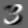
\includegraphics[width=\textwidth]{figs/pc1.jpg}
            \caption{PC1}
            \label{fig:pc1}
    \end{subfigure}
    \begin{subfigure}[b]{0.1\textwidth}
            \centering
            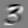
\includegraphics[width=\textwidth]{figs/pc2.jpg}
            \caption{PC2}
            \label{fig:pc2}
    \end{subfigure}
    \begin{subfigure}[b]{0.1\textwidth}
            \centering
            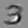
\includegraphics[width=\textwidth]{figs/pc3.jpg}
            \caption{PC3}
            \label{fig:pc3}
    \end{subfigure}
    \begin{subfigure}[b]{0.1\textwidth}
            \centering
            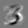
\includegraphics[width=\textwidth]{figs/pc4.jpg}
            \caption{PC4}
            \label{fig:pc4}
    \end{subfigure}
    \begin{subfigure}[b]{0.1\textwidth}
            \centering
            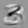
\includegraphics[width=\textwidth]{figs/pc5.jpg}
            \caption{PC5}
            \label{fig:pc5}
    \end{subfigure}
    \begin{subfigure}[b]{0.1\textwidth}
            \centering
            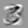
\includegraphics[width=\textwidth]{figs/pc6.jpg}
            \caption{PC6}
            \label{fig:pc6}
    \end{subfigure}
    \label{fig:pcs}
    \caption{Principal components of the set of threes.}
\end{figure*}
\begin{figure*}
    \centering
    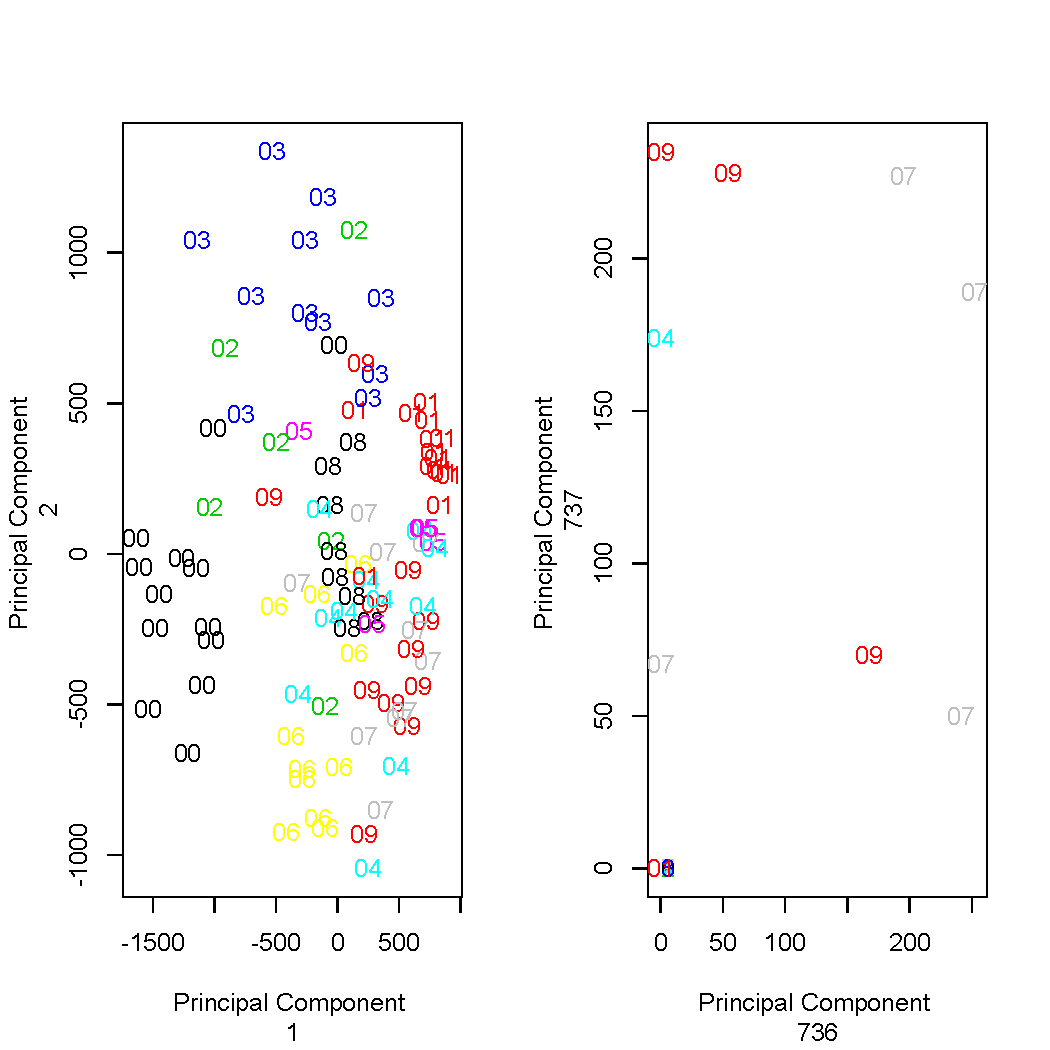
\includegraphics{PCAComponentPlot.pdf}
    \caption{(Left) Plot of images' first two principal components. (Right) Plot of images' two arbitrary pixel values}
    \label{fig:pcaplot}
\end{figure*}
\begin{figure*}
    \centering
    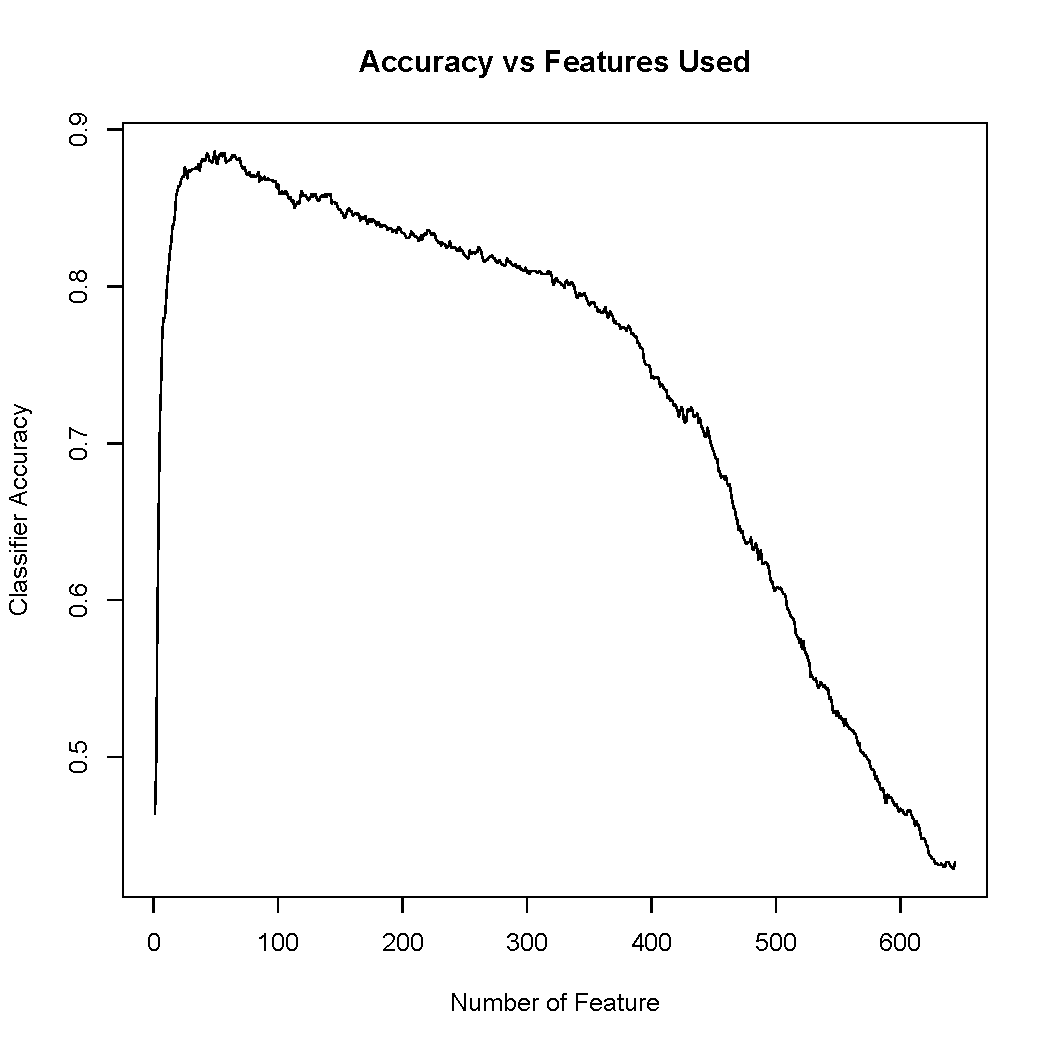
\includegraphics{figs/accuracyvsfeatures.pdf}
    \caption{Accuracy vs. number of features used in classification}
\end{figure*}
% section results (end)

\section{Discussion}
\subsection{Procedure Evaluation}
\label{subsec:eval}

Overall, our general implementation successfully addressed the issue of using PCA for hand-writing classification in a relatively simple and straight-forward way. Similar to other machine learning applications, the project called for the use of  \emph{supervised learning} (due to its use of data training and testing), a process that we correctly implemented from previously existing pseudo code and examples. Additionally, in regards to the computations associated with the training and PCA (outlined in the Methods section), much of it was performed using R's built-in functions which not only abstracted much of the much of the complexity but returned results with extremely low possibilities of error (lots of updates and implementation of the methods by many others guaranteed no systematic errors). Finally, because of the application of Bayesian statistics and conditional probability, both calculation and interpretation of the data was simplified, leaving the result to be one final probability representing the product of probabilities. 

The only limitations of this entire procedure dealt with the properties of the employed handwritten digit data as well as the intricacies of R's functional language. While we were able to perform the procedure on 60,000 images from the MNIST database, we were unable to perform the same operation using more test data or images from other databases (which would have been helpful in determining the threshold for data training and component quantity analysis). Also, much of the time spent on this project dealt with configuring the database's data into a collection with the right properties that would be either accepted by the functions or would result in any output (as incorrect specifications would result in an error or incorrect data that deviated from the available specification).

\subsection{Result Comparison}
\label{subsec:comparison}

Compared to our expectations made from the start of this project, the results obtained from this project were slightly better. With the general knowledge that the Naive-Bayes classifier could predict fairly well due to its elimination of high-dimensionality properties and simple probability mapping, we had assumed that our method could predict a maximum of 80-85\% of the images regardless of the number of components used. However, as observed from the results, our prediction range was comparably off as the percentage range varied considerably depending on the number of components used. For example, when using the first 50 and 100 components, the accuracy percentage was respectively 93\% and 92\%, both of which were a little higher than our maximum prediction rate. Conversely, when using zero or all 784 components, the accuracy percentage was around 66\%, a rate considerably worse than our initial guess.

\begin{figure*}
    \centering
    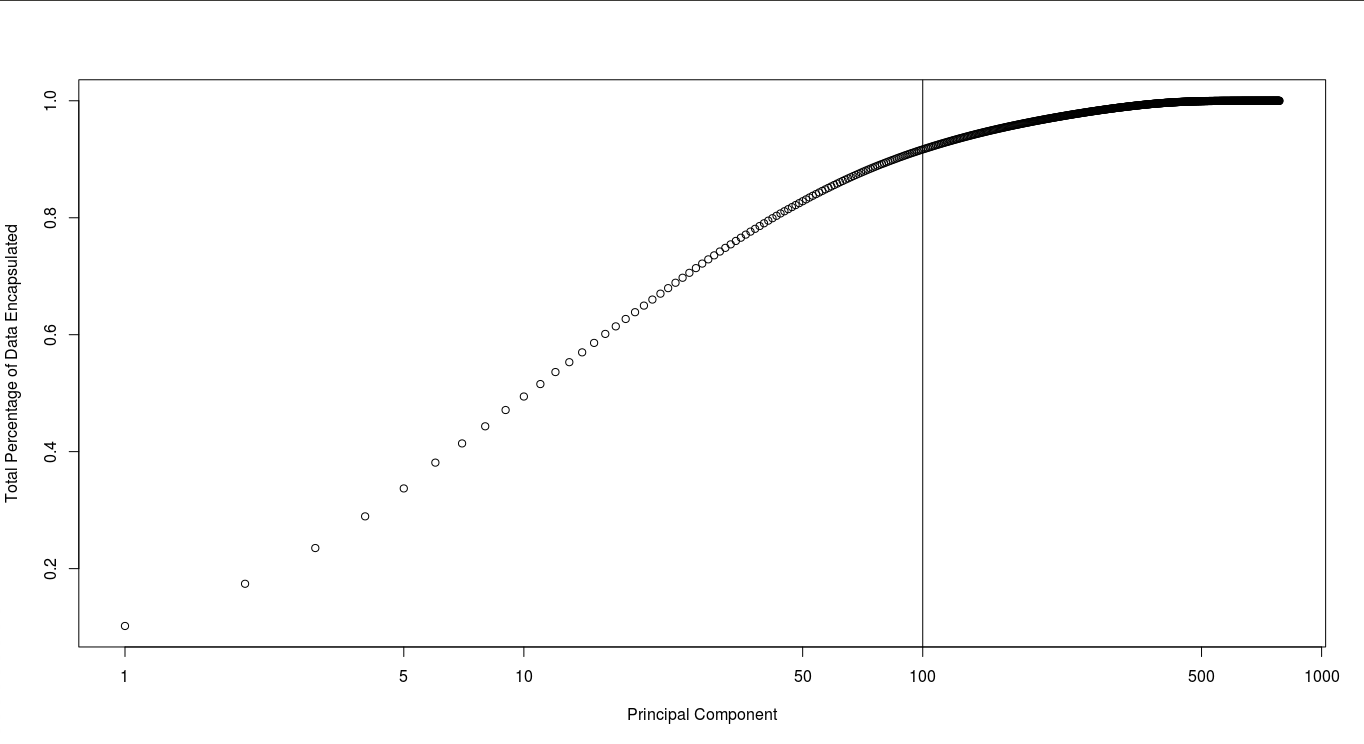
\includegraphics[scale=0.35]{CmptPctPlot.png}
    \caption{Cumulative Principal Component Numbers vs. Total Percent of Data}
\end{figure*}

The difference in findings also pertained to comparisons with other results obtained from similar PCA-applied Naive-Bayes classification. When compared to the STAT391 hand-writing classification model (discussed in-class), our procedure did a little better all-around as we were able to accurately predict more images. From Hil Lyons, we found that our resulted modeled the general pattern obtained by his results (with the maximum accuracy values obtained using ~100 components). However, our accuracy numbers were slightly higher, with our model accurately predicting 2-10\% more images than the model. Also, when compared to other groups' findings, we found that the accuracy rating model was again similar, with the maximum overall accuracy topped around 100 features. In addition, the accuracy rating quantity for these ranges modeled similarly to our results, loosely modeling a quadratic function with a maximum accuracy rating of around 92\%. The only difference between our results and their results were the accuracy percentages using extreme number of features. We found that our minimum accuracy values were higher than those observed by other groups, a range that was between 12\% at the lowest and 43\% at the highest. These differences in overall accuracy values could be attributed to two features: one being the limited training data that was used (only used a subset of the whole MNIST images) and the other being the use of R's built-in libraries.

\subsection{Potential Next Steps}
\label{subsec:next steps}

One possible next step would be to compare the Naive-Bayes classifier results with other classifier algorithms. The Naive-Bayes classifier, while an extension of Bayesian statistics, is one out of the many as a \emph{linear classifiers} as it determines the classification based on a linear combination of certain features. However, as explained before, the naïve assumption serves only as a extremely general model due to its naïve assumption of conditional independence across each of the given features (which most likely isn't the case). Thus, other linear classifiers such as logistic regression or the perceptron algorithm (both of which can be applied on the PCA-transformed data) as well as non-linear algorithms such as the K-nearest Neighbor algorithm (which classifies based on the total difference between features) can be compared against one another to determine the most accurate classification algorithm and, more importantly, if the Naive-Bayes algorithm stands alone in its ability to accurately determine handwritten digits.

Another possible step would be to utilize other distribution models or variations of the used Gaussian model when trying to statistically compare the test images' values with the training images' values for each of the top selected components. Each of the top computed components for each test image was modeled under a Gaussian distribution in order to determine the likelihood of obtaining that image based on these values. However, besides the normal distribution, there are other different distributions that have similar properties that could be used to estimate the probability of getting a certain pixel value such as the binomial (when used in a fashion similar to HW\#7), Cauchy, and Rayleigh distributions that might better classify the test images. Also, further comparisons under a multivariate normal distribution pose as a future possibility to further this project. In order to simplify the scope of this project, we assumed that each pixel value independently modeled under a one-dimensional normal distribution (in accordance to the conditional independence assumption). Unfortunately, this overall relationship between pixels is generally not independent, instead being correlated to other surrounding pixels. Thus, further testing might include comparisons of the accuracy results under a univariate normal distribution with those under a multivariate normal distribution (which starting code is attached at the end of this paper). 

Finally, the last possible addition to this project would be to compare the pre-made functions used in this project with similar self-implemented versions. Initially, we tried implementing the Naive-Bayes classifier as well as several methods that pertained to the PCA process (mainly the functions that would determine the transpose and covariance matrices). However, as mentioned in earlier sections, these functions actually contained many errors and required lots of time to implement correctly (for project legacy, these are attached to the end of this paper). Thus, it might be a worthwhile endeavor to compare the accuracy of these two methods and, if they don't output similar results, determine difference between R's implementation and user-generated methods.

% section discussion (end)

\bibliographystyle{plain}
\bibliography{stat}

\onecolumn
\appendix
\section{PCA.R}

\verbatiminput{PCA.R}

\section{MLE.R}

\verbatiminput{MLE.R}


\end{document}
